% Sumarização da execução de produção de 29/10/2026 (DATA_PRP_20C, 3 experimentos).
% Tabelas e figuras: docs/gap-analysis/production-run-20261029/completo/generate_report.py
%   (gera generated/*.tex e figures/production-run-*.pdf).

\documentclass[11pt,a4paper]{article}

\usepackage[T1]{fontenc}
\usepackage[utf8]{inputenc}
\usepackage[brazil]{babel}
\usepackage{amsmath,amssymb}
\usepackage{booktabs}
\usepackage{geometry}
\usepackage{hyperref}
\usepackage{enumitem}
\usepackage{graphicx}
\usepackage{float}

\geometry{margin=2.5cm}
\hypersetup{colorlinks=true,linkcolor=blue,urlcolor=blue}

\newcommand{\nTasks}{900}
\newcommand{\nCommon}{894}
\newcommand{\nClean}{446}
\newcommand{\nMissingC}{6}
\newcommand{\nCtasks}{894}
\newcommand{\nAfallback}{342}
\newcommand{\nBfallback}{318}
\newcommand{\pctAfallback}{38}
\newcommand{\pctBfallback}{35}
\newcommand{\nAgap}{558}
\newcommand{\nBgap}{582}
\newcommand{\pctBgainRejected}{10,9}

\newcommand{\boundDiffMedian}{0,00\%}
\newcommand{\boundDiffMean}{-0,02\%}


\title{Execução de Produção de 29/10/2026\\
       Impacto dos Métodos e Desempenho do Gap}
\author{Implementação do repositório LSVRP}
\date{\today}

\begin{document}

\maketitle

\begin{abstract}
\sloppy
Este documento resume a primeira execução de produção no cluster: três
experimentos sobre as instâncias de 20 clientes (\nTasks{} tarefas por experimento), com 1 thread e 3600~s de
orçamento total por tarefa. A análise segue duas frentes: (i) o impacto dos
diferentes métodos sobre a solução obtida e (ii) o desempenho do gap. Em
\pctAfallback\% e \pctBfallback\% das tarefas dos fluxos com MIP a solução do
MIP foi descartada na validação e a solução da heurística foi mantida; por isso
os resultados são apresentados em três visões (reportado, subconjunto limpo e
incumbente do MIP) e as conclusões são condicionadas a esse viés.
\end{abstract}

\section{Execução}

\subsection{Experimentos}

Todos usam as 150 instâncias de \texttt{DATA\_PRP\_20C}, os 6 vetores de peso de
\texttt{WEIGHTS\_OPTIMIZE} e $\alpha=0{,}99$, o modelo sem índice de veículo,
\texttt{objective\_scale}~$=10^{5}$, 1 thread, orçamento de 3600~s por tarefa (PSO ou
matheurística, construção do modelo e MIP) e commit \texttt{83b8f6}. As
configurações gravadas em \texttt{run\_configs} de cada \texttt{union\_results}
foram conferidas.

\begin{itemize}[leftmargin=*]
  \item \textbf{A} (\texttt{pso\_mip\_polish}): PSO (1000 iterações) seguido do MIP completo,
  com \emph{solution polishing} a partir de 3000~s.
  \item \textbf{B} (\texttt{matheuristic\_mip\_polish}): matheurística com start PSO
  (TSP 10~s, estágio restrito 180~s) seguida do MIP completo, com polishing a partir
  de 3000~s.
  \item \textbf{C} (\texttt{matheuristic}): matheurística com start PSO, estágio
  restrito até o fim do orçamento (3600~s), sem MIP completo.
\end{itemize}

\begin{table}[H]
  \centering
  \small
  \resizebox{\textwidth}{!}{\begin{tabular}{lrrrrr}
\toprule
Experimento & Tarefas & Faltantes & Solução final do MIP & Tempo mediano (min) & Tempo máximo (min) \\
\midrule
A. PSO + MIP & 900 & 0 & 558 & 51,8 & 55,3 \\
B. Matheurística + MIP & 900 & 0 & 582 & 60,0 & 60,0 \\
C. Matheurística & 894 & 6 & -- & 60,0 & 60,0 \\
\bottomrule
\end{tabular}
}
  \caption{Resumo da execução. ``Solução final do MIP'' conta as tarefas cujo
  resultado reportado vem do MIP. O tempo é o \texttt{solver\_time} do
  componente que produziu a solução final (no fluxo A, o tempo do PSO quando o MIP
  é descartado); a tarefa inteira usou até 60 minutos.}
  \label{tab:execucao}
\end{table}

\subsection{Status 1 do MPI}

O status 1 não indica queda do job. O runner de experimentos marca como
incompleto o experimento que termina com menos tarefas que o esperado e encerra
com código 1: o experimento C ficou com \nCtasks{} de \nTasks{} tarefas. Os
experimentos A e B estão completos (900 de 900) e nenhum \texttt{solver\_time}
reportado excede 3600~s.

As \nMissingC{} tarefas ausentes em C têm o arquivo de resultado com zero linhas:
a incumbente do estágio restrito foi rejeitada na validação
(\texttt{Produção/setup/capacidade}), e a matheurística não devolveu solução.

\begin{itemize}[leftmargin=*]
  \item \texttt{PRP24\_C20\_P8\_V5\_T12\_S3.dat}, pesos (0,25; 0,25; 0,25; 0,125; 0,125)
  \item \texttt{PRP24\_C20\_P8\_V5\_T12\_S5.dat}, pesos (0,2; 0,5; 0,1; 0,1; 0,1)
  \item \texttt{PRP25\_C20\_P8\_V5\_T12\_S1.dat}, pesos (0,2; 0,2; 0,2; 0,2; 0,2)
  \item \texttt{PRP27\_C20\_P8\_V5\_T12\_S1.dat}, pesos (0,3; 0,3; 0,1; 0,2; 0,1)
  \item \texttt{PRP29\_C20\_P8\_V5\_T12\_S2.dat}, pesos (0,35; 0,35; 0,1; 0,1; 0,1)
  \item \texttt{PRP8\_C20\_P8\_V5\_T12\_S1.dat}, pesos (0,35; 0,35; 0,1; 0,1; 0,1)
\end{itemize}


\section{Validade dos resultados}
\label{sec:validade}

Nos fluxos A e B, o resultado final só é o do MIP se a solução do CPLEX passa
na validação do projeto (\texttt{validate\_variables}); caso contrário, a solução
da heurística é mantida em silêncio e o gap fica vazio.

\begin{itemize}[leftmargin=*]
  \item Fluxo A: \nAfallback{} de \nTasks{} tarefas (\pctAfallback\%) ficaram com a solução do PSO.
  \item Fluxo B: \nBfallback{} de \nTasks{} tarefas (\pctBfallback\%) ficaram com a solução da
  matheurística. Os registros de estágio mostram o motivo nas \nBfallback{}:
  \emph{Rota desconectada da planta} na solução do MIP.
  \item Nessas tarefas, a solução do MIP era melhor que a mantida em \pctBgainRejected\%
  na média (Tabela~\ref{tab:ganho-mip}).
  \item O experimento A não grava registros de estágio, então os valores do MIP
  das \nAfallback{} tarefas descartadas não podem ser recuperados. Para B eles estão
  disponíveis (\texttt{exact\_start}).
  \item Não sabemos se a rota desconectada é um defeito real do modelo ou um
  artefato de tolerância da validação: as soluções rejeitadas não foram salvas.
\end{itemize}

Por isso as análises usam três visões:
\begin{description}[leftmargin=1.5em,style=nextline]
  \item[Reportado] o que está no \texttt{union\_results} (mistura soluções do MIP e da heurística);
  \item[Subconjunto limpo] as \nClean{} tarefas em que o MIP foi aceito em A e em B (e que existem em C);
  \item[Incumbente do MIP (B)] os valores de objetivo, limite e gap do estágio \texttt{exact\_start}
  de B, para as 900 tarefas, supondo válidas as soluções rejeitadas (não verificado).
\end{description}

\section{Frente (i): impacto dos métodos na solução}

\subsection{Distribuição da função objetivo}

Os valores de FO só são comparáveis entre métodos para o mesmo vetor de pesos
(cada vetor define um objetivo diferente); as médias globais abaixo servem de
referência geral.

\begin{table}[H]
  \centering
  \small
  \begin{tabular}{lrrrrrr}
\toprule
Fluxo & n & Média & Mediana & P10 & P90 & Máx. \\
\midrule
A. PSO + MIP (reportado) & 900 & 0,2749 & 0,2622 & 0,2143 & 0,3582 & 0,4832 \\
B. Matheurística + MIP (reportado) & 900 & 0,2751 & 0,2636 & 0,2124 & 0,3608 & 0,4945 \\
B. Matheurística + MIP (incumbente do MIP) & 900 & 0,2638 & 0,2503 & 0,2025 & 0,3487 & 0,4945 \\
C. Matheurística & 894 & 0,2669 & 0,2544 & 0,2042 & 0,3481 & 0,4926 \\
\bottomrule
\end{tabular}

  \caption{FO por fluxo, todas as tarefas disponíveis (menor é melhor).}
  \label{tab:fo-dist}
\end{table}

\begin{table}[H]
  \centering
  \small
  \begin{tabular}{lrrrr}
\toprule
Fluxo & Média & Mediana & P10 & P90 \\
\midrule
A. PSO + MIP & 0,2650 & 0,2525 & 0,2024 & 0,3469 \\
B. Matheurística + MIP & 0,2666 & 0,2526 & 0,2062 & 0,3484 \\
C. Matheurística & 0,2676 & 0,2534 & 0,2043 & 0,3476 \\
\bottomrule
\end{tabular}

  \caption{FO no subconjunto limpo (\nClean{} tarefas, MIP aceito em A e em B).}
  \label{tab:fo-clean}
\end{table}

No subconjunto limpo os três fluxos são praticamente equivalentes: a diferença
entre as médias é de cerca de 1\%. A vantagem aparente do fluxo C na média geral
(Tabela~\ref{tab:fo-dist}) vem do descarte do MIP em A e em B, e não de uma
qualidade superior da matheurística.

\subsection{Comparações pareadas}

Diferença relativa $(\mathrm{FO}_1-\mathrm{FO}_2)/\mathrm{FO}_2$ por tarefa; valores negativos
indicam que o primeiro fluxo é melhor. O intervalo de confiança vem de
\emph{bootstrap} (4000 reamostragens) da média da diferença.

\begin{table}[H]
  \centering
  \scriptsize
  \begin{tabular}{lrrrrrr}
\toprule
Comparação (1º contra 2º) & n & 1º melhor & Empate & Mediana & Média & IC 95\% da média \\
\midrule
A contra B & 894 & 65\% & 0\% & -0,11\% & 0,49\% & [-0,19\%; 1,20\%] \\
A contra C & 894 & 35\% & 0\% & 1,33\% & 4,06\% & [3,14\%; 4,97\%] \\
B contra C & 894 & 27\% & 8\% & 1,23\% & 4,04\% & [3,18\%; 4,93\%] \\
B (MIP) contra C & 894 & 43\% & 1\% & 0,30\% & -0,54\% & [-1,26\%; 0,15\%] \\
A contra B (MIP) & 894 & 38\% & 0\% & 0,76\% & 5,03\% & [4,23\%; 5,86\%] \\
\bottomrule
\end{tabular}

  \caption{Comparação pareada nas \nCommon{} tarefas presentes nos três experimentos.}
  \label{tab:pareada-todas}
\end{table}

\begin{table}[H]
  \centering
  \scriptsize
  \begin{tabular}{lrrrrrr}
\toprule
Comparação (1º contra 2º) & n & 1º melhor & Empate & Mediana & Média & IC 95\% da média \\
\midrule
A contra B & 446 & 60\% & 0\% & -0,19\% & -0,33\% & [-0,97\%; 0,31\%] \\
A contra C & 446 & 46\% & 0\% & 0,22\% & -0,16\% & [-1,23\%; 1,01\%] \\
B contra C & 446 & 41\% & 2\% & 0,38\% & 0,35\% & [-0,71\%; 1,46\%] \\
\bottomrule
\end{tabular}

  \caption{Comparação pareada no subconjunto limpo (\nClean{} tarefas).}
  \label{tab:pareada-limpo}
\end{table}

\begin{figure}[H]
  \centering
  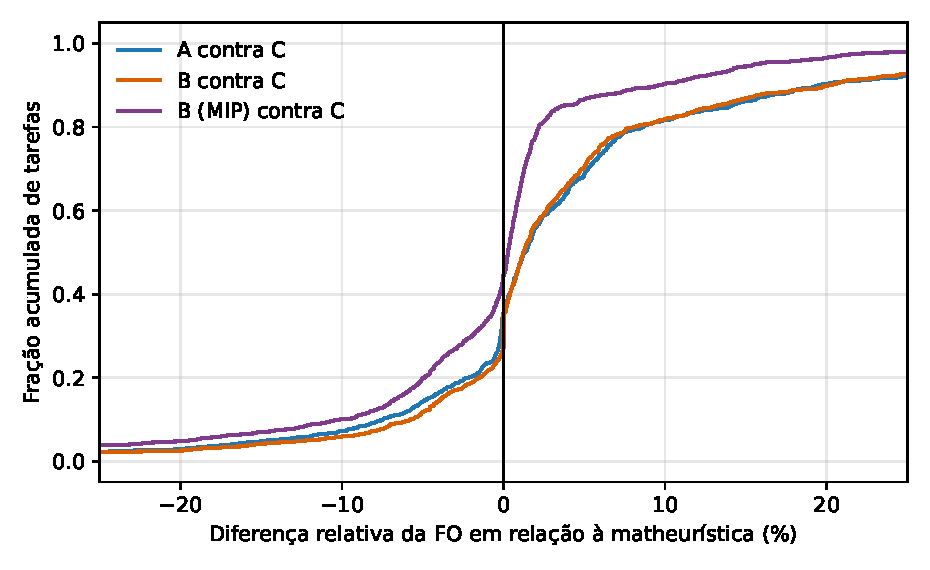
\includegraphics[width=0.8\textwidth]{figures/production-run-fo-diff-cdf.pdf}
  \caption{Distribuição acumulada da diferença relativa da FO em relação à
  matheurística (fluxo C), nas \nCommon{} tarefas comuns. Valores à esquerda de zero
  indicam que o fluxo é melhor que C.}
  \label{fig:fo-diff}
\end{figure}

\begin{itemize}[leftmargin=*]
  \item No subconjunto limpo nenhuma diferença é distinguível de zero: todos os
  intervalos de confiança incluem 0 e as médias ficam entre $-0{,}3\%$ e $+0{,}4\%$.
  \item Com os valores reportados, A e B parecem pior que C em média (cerca de
  $+4\%$), mas esse efeito desaparece ao usar a incumbente do MIP em B
  (B~(MIP) contra C: $-0{,}5\%$, intervalo que inclui 0).
  \item A contra B não se distingue: o desempenho dos dois fluxos com MIP é
  semelhante, e o ponto de partida (PSO ou matheurística) não muda o resultado
  de modo mensurável.
\end{itemize}

\subsection{Por vetor de pesos e por classe de instância}

\begin{table}[H]
  \centering
  \small
  \begin{tabular}{lrrrr}
\toprule
Pesos $w_1,\ldots,w_5$ & A (reportado) & B (reportado) & B (MIP) & C \\
\midrule
(0,2; 0,2; 0,2; 0,2; 0,2) & 0,2580 & 0,2614 & 0,2552 & 0,2611 \\
(0,2; 0,5; 0,1; 0,1; 0,1) & 0,3611 & 0,3606 & 0,3519 & 0,3496 \\
(0,25; 0,25; 0,25; 0,125; 0,125) & 0,2443 & 0,2431 & 0,2156 & 0,2325 \\
(0,3; 0,3; 0,1; 0,1; 0,2) & 0,2632 & 0,2638 & 0,2569 & 0,2606 \\
(0,3; 0,3; 0,1; 0,2; 0,1) & 0,2506 & 0,2486 & 0,2420 & 0,2381 \\
(0,35; 0,35; 0,1; 0,1; 0,1) & 0,2726 & 0,2729 & 0,2609 & 0,2597 \\
\bottomrule
\end{tabular}

  \caption{FO média por vetor de pesos. Só as colunas de uma mesma linha são
  comparáveis. ``B (MIP)'' usa a incumbente do MIP de B para as 900 tarefas.}
  \label{tab:fo-peso}
\end{table}

\begin{table}[H]
  \centering
  \small
  \begin{tabular}{lrrrr}
\toprule
Classe & A (reportado) & B (reportado) & B (MIP) & C \\
\midrule
1 & 0,2710 & 0,2722 & 0,2636 & 0,2636 \\
2 & 0,2808 & 0,2793 & 0,2660 & 0,2722 \\
3 & 0,2731 & 0,2737 & 0,2616 & 0,2649 \\
\bottomrule
\end{tabular}

  \caption{FO média por classe de instância.}
  \label{tab:fo-classe}
\end{table}

O melhor fluxo depende do vetor de pesos: B~(MIP) é o menor em 3 dos 6 vetores e
C em outros 3. A classe 2 tem a maior FO média nos quatro conjuntos de valores e
as diferenças entre fluxos dentro de cada classe são pequenas.

\subsection{Composição da solução}

\begin{table}[H]
  \centering
  \small
  \begin{tabular}{lrrr}
\toprule
Componente (média por tarefa) & A & B contra A & C contra A \\
\midrule
f1 (produção) & 19 073 660 & -0,0\% & 0,0\% \\
f2 (setup) & 18 484 & 0,4\% & 4,1\% \\
f3 (estoque) & 787 164 & -0,3\% & 5,0\% \\
f4 (transp. fixo) & 1 507 753 & 0,1\% & -3,8\% \\
f5 (transp. variável) & 97 070 & 1,8\% & -3,7\% \\
nº de setups (soma de $y$) & 427,9 & 0,2\% & 2,7\% \\
\bottomrule
\end{tabular}

  \caption{Média dos totais de cada componente de custo no horizonte, no
  subconjunto limpo, e variação relativa dos fluxos B e C em relação a A.}
  \label{tab:componentes}
\end{table}

As soluções de A e B têm composição muito parecida (diferenças de até 2\%). A matheurística (C) troca custo de
transporte por setup e estoque: cerca de 4\% menos transporte fixo e variável
(f4 e f5), contra 4\% a 5\% mais setup e estoque (f2 e f3) e 2,7\% mais setups.
O custo de produção (f1) é o mesmo nos três: é o mínimo físico dado pela demanda.

\subsection{Quanto o MIP melhora a matheurística}

Em B, o estágio \texttt{exact\_start} parte da solução do estágio restrito da
matheurística. A Tabela~\ref{tab:ganho-mip} mostra a melhora relativa da FO que o
MIP obteve em 3600~s menos o tempo da matheurística.

\begin{table}[H]
  \centering
  \small
  \begin{tabular}{lrrrrr}
\toprule
Grupo & n & Média & Mediana & P90 & Máx. \\
\midrule
Solução do MIP aceita & 582 & 9,7\% & 5,4\% & 25,6\% & 43,2\% \\
Solução do MIP rejeitada & 318 & 10,9\% & 5,9\% & 26,6\% & 40,3\% \\
Todas & 900 & 10,1\% & 5,7\% & 26,2\% & 43,2\% \\
\bottomrule
\end{tabular}

  \caption{Melhora relativa da FO do MIP sobre a solução do estágio restrito da
  matheurística (B), por tarefa.}
  \label{tab:ganho-mip}
\end{table}

O MIP melhora a solução do estágio restrito de 180~s em mediana de 5,7\%, com
cauda de até 43\%. A matheurística sozinha com 3600~s no estágio restrito
(fluxo C) fica, no subconjunto limpo, a 0,4\% de B (Tabela~\ref{tab:pareada-limpo}),
sem diferença distinguível: dar mais tempo ao estágio restrito rende
aproximadamente o mesmo que passar ao MIP completo. A comparação mistura tempo e
método, então não separa os dois efeitos.

\section{Frente (ii): desempenho do gap}

\subsection{Disponibilidade e distribuição}

O gap só existe quando o resultado final é do MIP: \nAgap{} tarefas em A,
\nBgap{} em B (reportado) e as 900 em B se usarmos o estágio \texttt{exact\_start}.
O fluxo C não tem gap por construção.

\begin{table}[H]
  \centering
  \scriptsize
  \resizebox{\textwidth}{!}{\begin{tabular}{lrrrrrrrrr}
\toprule
Fonte do gap & n & Média & Mediana & P90 & Máx. & $\le 5\%$ & $\le 10\%$ & $\le 20\%$ & Gap $0$ \\
\midrule
A (reportado, MIP aceito) & 558 & 16,2\% & 11,0\% & 36,9\% & 55,8\% & 20\% & 47\% & 68\% & 1 \\
B (reportado, MIP aceito) & 582 & 16,5\% & 11,1\% & 36,4\% & 60,3\% & 19\% & 46\% & 67\% & 2 \\
B (MIP, todas as tarefas) & 900 & 15,1\% & 10,1\% & 34,2\% & 60,3\% & 20\% & 50\% & 72\% & 2 \\
A (subconjunto limpo) & 446 & 16,5\% & 11,6\% & 36,3\% & 54,6\% & 19\% & 46\% & 66\% & 1 \\
B (subconjunto limpo) & 446 & 16,9\% & 11,3\% & 36,7\% & 54,6\% & 19\% & 46\% & 64\% & 2 \\
\bottomrule
\end{tabular}
}
  \caption{Distribuição do gap. As colunas ``$\le x\%$'' são a fração de tarefas
  com gap menor ou igual a $x$; ``Gap 0'' é o número de tarefas com otimalidade provada.}
  \label{tab:gap-dist}
\end{table}

\begin{figure}[H]
  \centering
  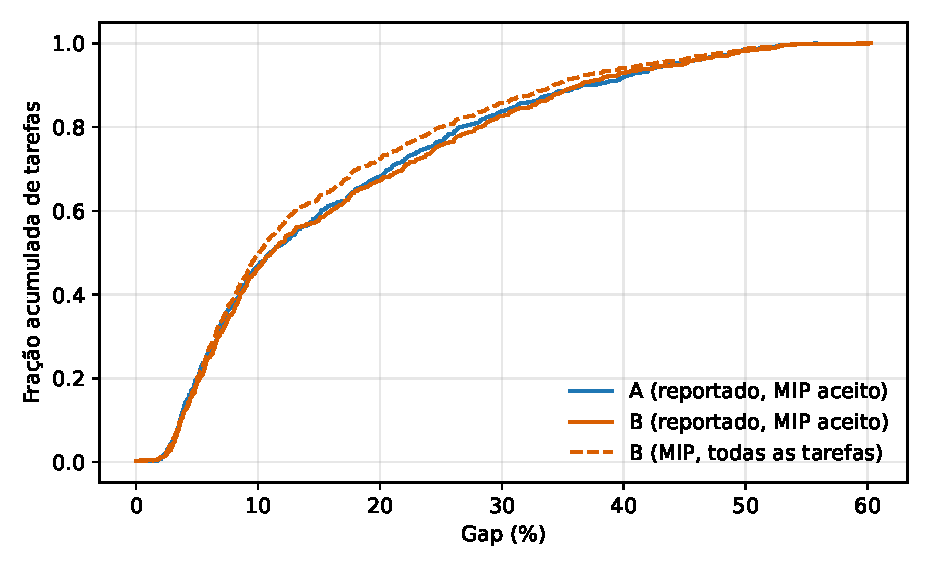
\includegraphics[width=0.8\textwidth]{figures/production-run-gap-cdf.pdf}
  \caption{Distribuição acumulada do gap.}
  \label{fig:gap-cdf}
\end{figure}

\begin{itemize}[leftmargin=*]
  \item O gap mediano é de cerca de 10\% a 11\% e a média de 15\% a 17\%. Metade das
  tarefas (50\% em B-MIP) fecha em 10\% ou menos; 67\% a 72\% ficam em 20\% ou menos.
  \item Só 1 a 2 tarefas (de 558--900) têm otimalidade provada (gap zero).
  \item O pior caso chega a 55\%--60\%.
\end{itemize}

\subsection{O limite inferior não depende do ponto de partida}

\begin{table}[H]
  \centering
  \small
  \begin{tabular}{lrrr}
\toprule
Fonte & Limite inferior médio & Incumbente média & Gap médio \\
\midrule
A (subconjunto limpo) & 0,2205 & 0,2650 & 16,5\% \\
B (subconjunto limpo) & 0,2206 & 0,2666 & 16,9\% \\
B (MIP, todas as tarefas) & 0,2237 & 0,2638 & 15,1\% \\
\bottomrule
\end{tabular}

  \caption{Limite inferior, incumbente e gap médios. O limite de A é derivado do
  gap reportado ($\mathrm{FO}\,(1-\mathrm{gap})$).}
  \label{tab:bound}
\end{table}

No subconjunto limpo o limite inferior médio é o mesmo em A e em B (0,2205 contra
0,2206; diferença mediana \boundDiffMedian{}). A diferença de gap entre os dois
fluxos vem então apenas da incumbente: o limite é determinado pela raiz do CPLEX
(laço de cortes) e não pelo start. Isso é coerente com o que se vê na análise
anterior: depois da raiz a árvore quase não eleva o limite.

\subsection{Por vetor de pesos e por classe}

\begin{table}[H]
  \centering
  \scriptsize
  \resizebox{\textwidth}{!}{\begin{tabular}{lrrrrrr}
\toprule
Pesos $w_1,\ldots,w_5$ & A (rep.) & B (rep.) & B (MIP) média & B (MIP) mediana & A sem MIP & B sem MIP \\
\midrule
(0,2; 0,2; 0,2; 0,2; 0,2) & 29,4\% & 29,6\% & 30,2\% & 32,8\% & 20\% & 21\% \\
(0,2; 0,5; 0,1; 0,1; 0,1) & 6,3\% & 7,0\% & 6,4\% & 4,9\% & 42\% & 45\% \\
(0,25; 0,25; 0,25; 0,125; 0,125) & 16,5\% & 17,2\% & 16,9\% & 13,9\% & 40\% & 40\% \\
(0,3; 0,3; 0,1; 0,1; 0,2) & 20,5\% & 20,6\% & 18,3\% & 15,0\% & 39\% & 30\% \\
(0,3; 0,3; 0,1; 0,2; 0,1) & 10,1\% & 10,5\% & 9,9\% & 7,8\% & 36\% & 31\% \\
(0,35; 0,35; 0,1; 0,1; 0,1) & 8,1\% & 8,6\% & 8,7\% & 6,8\% & 51\% & 45\% \\
\bottomrule
\end{tabular}
}
  \caption{Gap por vetor de pesos. ``A (rep.)'' e ``B (rep.)'' são os gaps reportados
  (só tarefas com MIP aceito); ``B (MIP)'' usa o estágio \texttt{exact\_start} das 900
  tarefas; ``sem MIP'' é a fração de tarefas em que a solução do MIP foi descartada.}
  \label{tab:gap-peso}
\end{table}

\begin{table}[H]
  \centering
  \scriptsize
  \resizebox{\textwidth}{!}{\begin{tabular}{lrrrrrr}
\toprule
Classe & A (rep.) & B (rep.) & B (MIP) média & B (MIP) mediana & A sem MIP & B sem MIP \\
\midrule
1 & 15,0\% & 16,4\% & 15,1\% & 10,8\% & 30\% & 30\% \\
2 & 18,4\% & 18,0\% & 16,1\% & 9,6\% & 41\% & 40\% \\
3 & 15,3\% & 15,0\% & 14,1\% & 10,0\% & 43\% & 37\% \\
\bottomrule
\end{tabular}
}
  \caption{Gap por classe de instância.}
  \label{tab:gap-classe}
\end{table}

\begin{itemize}[leftmargin=*]
  \item \textbf{O vetor de pesos explica a maior parte da variação do gap.} Com pesos
  iguais o gap médio é de cerca de 30\% (mediana 33\%); com mais peso em f2 ou em f1
  e f2 ($0{,}2;0{,}5;\ldots$ e $0{,}35;0{,}35;\ldots$) ele cai para 6\%--9\%. Não
  investigamos a causa; uma hipótese é que o peso maior nos custos fixos aumenta a parte do
  objetivo que o limite já enxerga bem, mas isso não foi testado.
  \item O descarte do MIP é menos frequente com pesos iguais (cerca de 20\%) e mais
  frequente nos demais vetores (30\% a 51\%); os gaps reportados nesses vetores
  têm, portanto, maior viés de seleção.
  \item Entre as classes de instância o gap médio varia pouco (14\%--18\%), com
  mediana em torno de 10\%.
\end{itemize}

\subsection{Ressalva sobre o significado do gap}

Os targets atuais tornam parte do objetivo irredutível: a soma dos targets de f1
fica abaixo do custo mínimo de produção em 100\% das instâncias de 20 e de 30
clientes, o que impõe $\lambda\ge 0{,}02$--$0{,}10$ (mediana $\approx 0{,}06$) a
qualquer solução. Limite e incumbente carregam essa mesma constante, de modo que o
gap relativo reportado fica achatado em relação ao que seria com targets
consistentes. Esse efeito foi estimado em análise anterior, não nesta execução.

\section{Conclusões e pontos em aberto}

\begin{enumerate}[leftmargin=*]
  \item A execução está completa para A e B e incompleta para C (6 tarefas).
  \item Em \pctAfallback\% (A) e \pctBfallback\% (B) das tarefas a solução do MIP foi descartada
  na validação. Antes de concluir sobre o ganho do MIP é preciso identificar se o
  defeito está no modelo sem índice de veículo, na tolerância da validação ou na
  reconstrução das rotas.
  \item No subconjunto limpo, PSO + MIP, matheurística + MIP e matheurística sozinha
  são equivalentes na FO (diferenças de até cerca de 1\%, todas dentro do intervalo
  de confiança).
  \item O limite inferior é o mesmo nos dois fluxos com MIP; o gap depende só da
  incumbente. O gap mediano é de cerca de 10\%--11\% e varia muito com o vetor de
  pesos (6\% a 30\%).
  \item Não foi possível isolar o efeito do polishing: nenhum experimento rodou sem ele.
\end{enumerate}

\paragraph{Próximos passos.}
\begin{itemize}[leftmargin=*]
  \item Reproduzir localmente uma tarefa rejeitada, salvar a solução do MIP e identificar a
  violação; depois refazer as tarefas afetadas e completar as 6 tarefas de C.
  \item Gravar nos resultados a solução rejeitada, o motivo e o gap do MIP mesmo quando a
  heurística é mantida.
  \item Retomada por tarefa, além da retomada por experimento.
  \item Reavaliar os targets (soma consistente, nadir sem prioridade) antes de novas execuções.
\end{itemize}

\end{document}
